\documentclass{paper}
\usepackage[utf8]{inputenc}

\title{Realidade Virtual}
\author{Carlos Eduardo Mendonça Clark}




\usepackage{natbib}
\usepackage{graphicx}

\begin{document}

\maketitle

\section{Introdução}
A ideia sobre Realidade Virtual(VR) nasceu a mais de 40 anos e o conceito por trás deste nome é a procura da imersão total do usuário em um ambiente virtual diferente ou igual ao real. Para isto, é utilizado alguns componentes para reproduzir os sentidos da visão e audição, uma espécie de óculos e um fone 7.1 são as chaves principais pra imersão total do usúario. Hoje em dia temos o próprio modelo comercial(Oculus Rift) que está sendo vendido para jogos e afins. Mas a ideologia completa da Realidade Virtual ainda não está completa e anda em desenvolvimento, já que em teoria busca-se a imersão total com os 5 sentidos em sintonia devem estar presentes no mundo virtual.
\begin{figure}[h!]
\centering
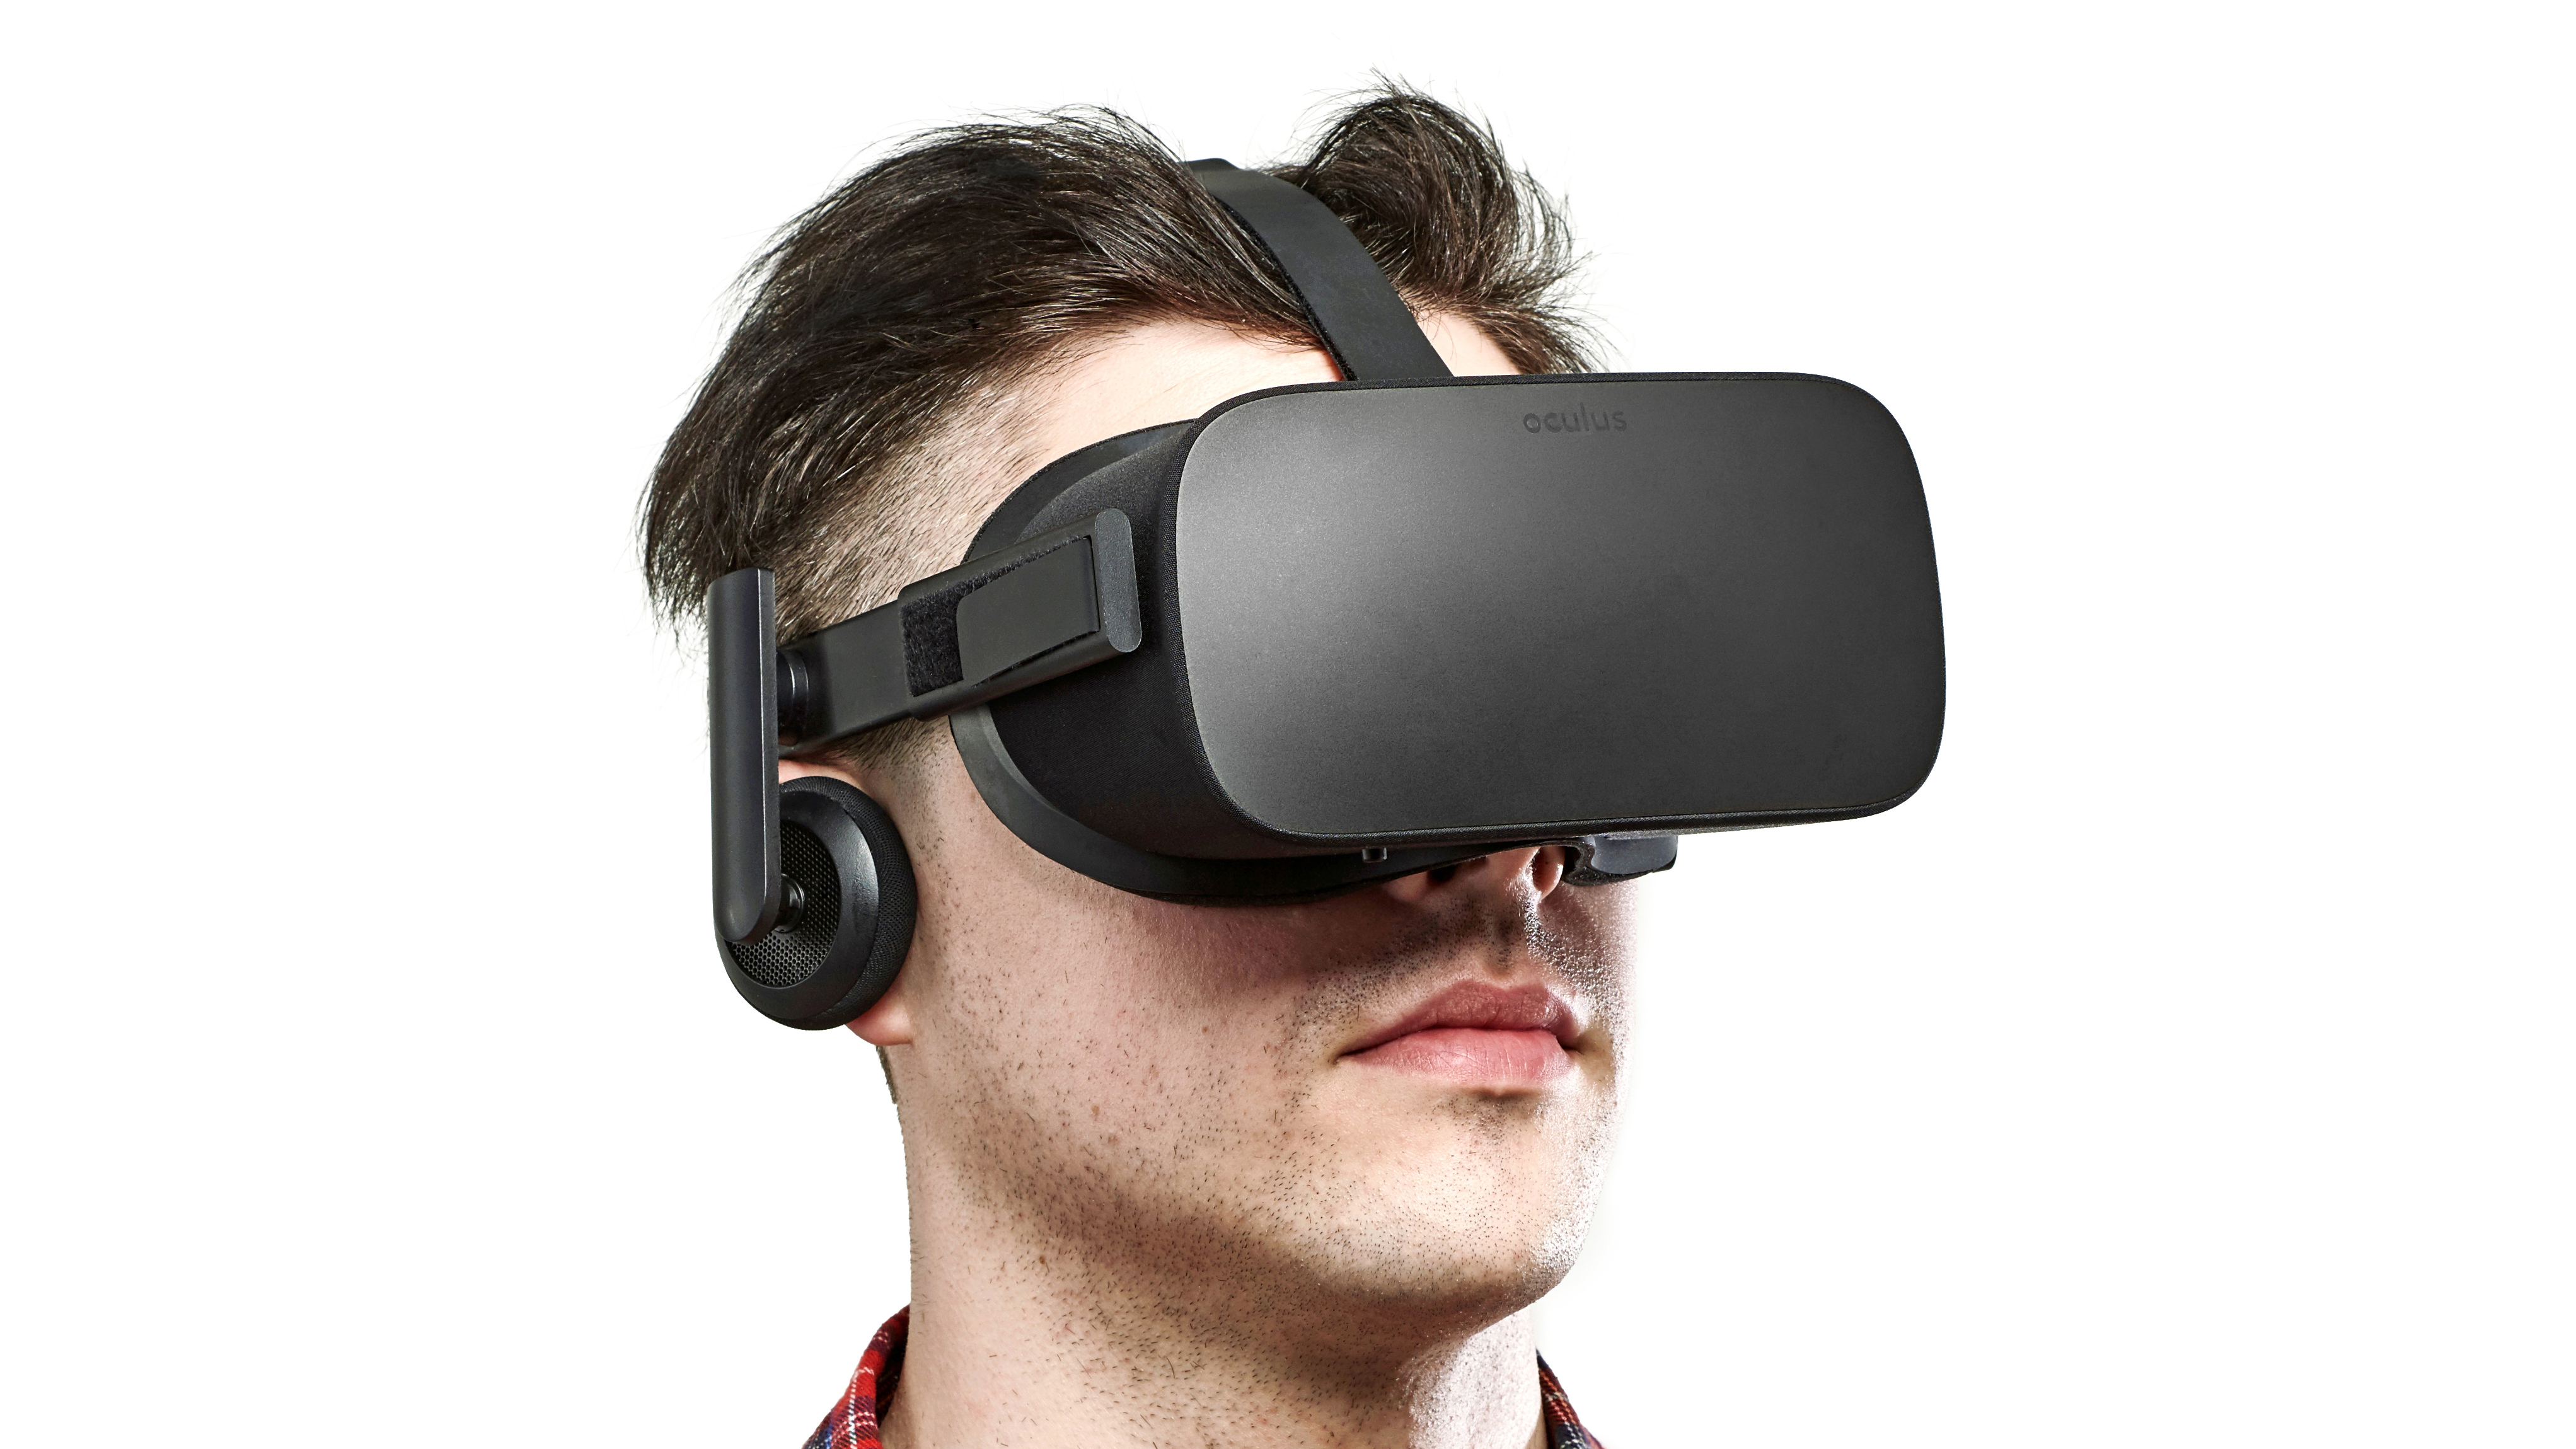
\includegraphics[scale=0.4]{Oculus.jpg}
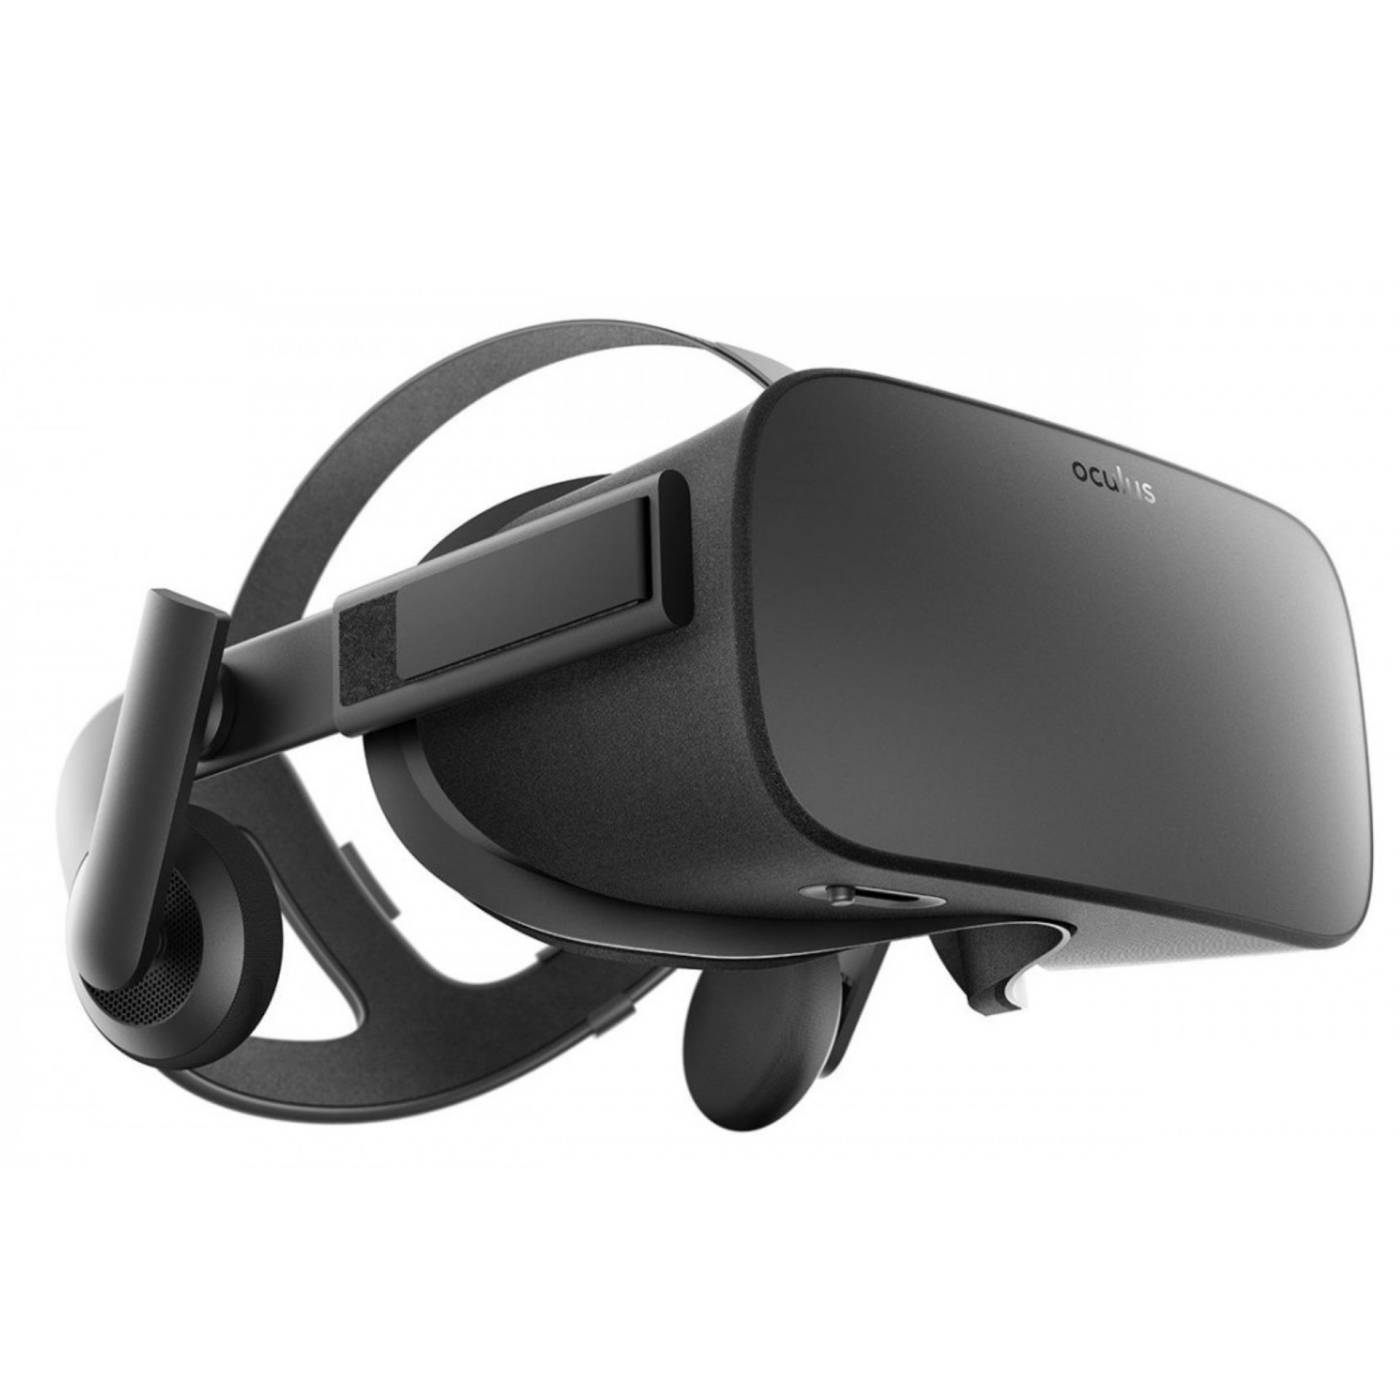
\includegraphics[scale=0.08]{Oculus2.jpg}
\caption{Oculus Rift\citep{Oculus}}

\end{figure}



\section{Relevância}
A cadeira de Realidade Virtual, apesar de ser eletiva, ela é super importante para abrir o leque de possibilidades de cada estudante para seguirem por uma área e com certeza Realidade Virtual é uma tecnologia que será de extremo uso no futuro próximo, por conta das possibilidades que se podem ter seja no meio estudantil\cite{Fonte2} (através de salas compostas em um ambiente virtual), lazer(talvez com a inovação do que conhecemos de cinemas ou jogos) e até mesmo social\cite{Fonte}(uma reunião, conversar e interagir com outras pessoas). Com essa disciplina os próprios alunos de hoje em dia podem ter a imaginação para construir este futuro. 
\section{Relações com outras disciplinas}
Definitivamente Realidade Virtual tem relação com várias disciplinas porém está mais interligada com Algebra(Matemática) e Design Gráfico. Indiscutivelmente, Algebra é necessário para o entendimento da criação deste ambiente virtual já que, em tese, estaria criando um mundo complexo novamente, para isso é necessário da algebra para aplicar a noção de perspectiva, criação de objetos "físicos" e etc. Já o Design Gráfico seria a implementação desse conhecimento no ambiente virtual, para moldar e renderizar tais ideias no mundo virtual.
\begin{figure}[h!]
\centering

\includegraphics[scale=0.24]{Jogador.png}
\caption{Filme e livro Jogador Num.1\cite{Fonte3}}
\end{figure}

\bibliographystyle{plain}
\bibliography{cemc.bib}



\end{document}
